%-------------------------------------------------------------
% CV in english
% Hugo Ferrando Seage - 2017
%-------------------------------------------------------------

\documentclass[a4paper, 12pt]{article}
\usepackage[utf8]{inputenc}
\usepackage[T1]{fontenc}
\usepackage[english]{babel}
\usepackage{subfig}
\usepackage{tabularx}
\usepackage{paracol}
\usepackage{booktabs}
\usepackage{enumitem} % Customize enumerate items
\usepackage{longtable} % Required to make tables span more than one page
\usepackage{graphicx} % Required for including pictures
\usepackage{multicol}
\usepackage[cm]{fullpage}
\usepackage[usenames,dvipsnames]{xcolor} % Required for specifying custom colors
\usepackage[pdfstartview=Fit]{hyperref} % Required for adding links	and customizing them
\definecolor{linkcolour}{rgb}{0,0.2,0.6} % Link color
\hypersetup{colorlinks,breaklinks,urlcolor=linkcolour,linkcolor=linkcolour, pdfpagemode=UseNone} % Set link colors throughout the document
\hyphenpenalty=10000
\setlength{\columnsep}{-3.5cm}

\newenvironment{myparacol}[2][]{%
\begin{paracol}{#2}[#1]\setlength{\parindent}{0pt}}{%
\end{paracol}}

\begin{document}
\pagestyle{empty} % Removes page numbering

\begin{flushright}
    Computer Science graduate\\
    +34 680 340 463\\
    \href{mailto: me@hugofs.com}{me@hugofs.com}\\
    \href{https://hugofs.com}{hugofs.com}\\
\end{flushright}

\vspace{-27mm}

\begin{figure}[ht!]
    \begin{flushleft}
        \subfloat{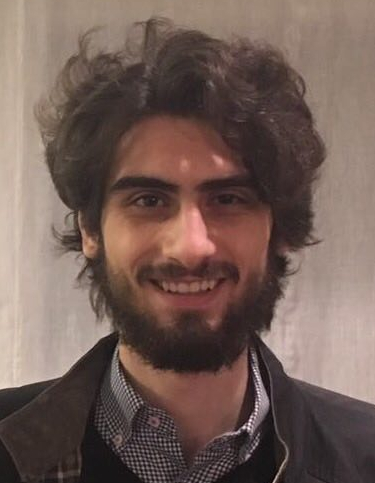
\includegraphics[width=0.13\textwidth]{images/hugo.jpg}}
    \end{flushleft}
\end{figure}

{\textsc {\Huge \vspace{5mm} \hspace{-13mm} Hugo Ferrando Seage}}\\

\setlength{\columnsep}{24pt}
\begin{sloppypar}
\begin{myparacol}{2}
    EDUCATION
    \vspace{1mm}
    \hrule
    \kern9pt
    \textbf{U-tad} \hfill 17 -- 18

    Master in graphics programming and simulation\\

    \textbf{Universidad Europea de Madrid} \hfill 14 -- 17

    Bachelor's Degree in Computer Science

    \textit{Thesis:} \href{https://github.com/hugo19941994/movie-pepper-doc/raw/master/thesis.pdf}{Natural language processing based film recommendation engine}

    \textit{Activities:} Robotics Club, Data Science Lab

    \textit{GPA:} 7.8/10\\

    \textbf{Universidad Politécnica de Madrid} \hfill 12 -- 14

    Bachelor's Degree in Computer Science

    \textit{Activities:} ACM Student Chapter
    \\

    \switchcolumn

    EXPERIENCE
    \vspace{1mm}
    \hrule
    \kern9pt

    \textbf{Telefónica I+D} \hfill dec 17 --

    Software Engineer for SmartDigits\\

    \textbf{Telefónica $\sim$ Talentum} \hfill sep 16 -- nov 17

    Several Telefónica I+D \& LUCA projects

    Recommendation engine improvements of Telefonica's video on demand service Movistar+\\

    \textbf{Product Hackers} \hfill jun 16 -- oct 16

    Development of web apps and chat bots using Angular 2 and Ionic 2 for mobile devices and the web\\

    \textbf{UEM} \hfill sep 15 -- mar 17

    \href{https://www.researchgate.net/publication/314142014_Prediction_of_User_Opinion_for_Products_-_A_Bag-of-Words_and_Collaborative_Filtering_based_Approach}{Prediction model of users and their opinion, based on Amazon review texts, using distributed computing}

    Motion detection of people swimming in pools and beaches using OpenCV

    \href{https://github.com/hugo19941994/infrac-coche}{Android app to detect, alert and register traffic violations using OpenCV}
    \\

    \switchcolumn

    TECHNICAL KNOWLEDGE
    \vspace{1mm}
    \hrule
    \kern9pt

    Python, C++, Go, Javascript ES7, Bash\\

    Apache Spark, React, Angular, Flask, OpenGL, Android SDK \& NDK\\

    GNU/Linux, Git, SSH, GPG, \LaTeX, Markdown, Nginx, Jenkins\\

    LANGUAGES
    \vspace{1mm}
    \hrule
    \kern9pt
    \noindent\begin{tabularx}{\columnwidth}{ @{} X X X }
        English & Spanish & Italian
    \end{tabularx}
    \\

    CERTIFICATIONS
    \vspace{1mm}
    \hrule
    \kern9pt
    Certificate in Advanced English (CAE)

    CCNA 1: Introduction to Networks

    CCNA 2: Routing and Switching Essentials

    CCNA 4: Connecting Networks

    \switchcolumn

    \noindent PROJECTS
    \vspace{1mm}
    \hrule
    \kern9pt
    \href{https://github.com/hugo19941994/SpaceInvaders-Emu}{Intel 8080 emulator}: Space Invaders emulator for MacOS written in C++ and OpenGL

    \href{https://github.com/hugo19941994/CHIP8-Emu}{CHIP-8 interpreter}: CHIP-8 emulator for Windows and Linux

    \href{https://vpn.hugofs.com}{ovpn}: OpenVPN based VPN provider

    \href{https://github.com/hugo19941994/ViajeFacil}{ViajeFácil}: Management software for flight agencies

    \href{https://github.com/hugo19941994/CV-Parser}{CV-Parser}: CV management system using Name Entity Recognition and bayesian networks

    \href{https://github.com/hugo19941994/robot}{Human Rescue Bot}: Laureate Awards for Excellence in Robotics Engineering 2016 1\textsuperscript{st} place winner

\end{myparacol}
\end{sloppypar}
\end{document}
